\subsubsection{Flow speed}
Figure \ref{fig:Ramp-Vel} shows the flow speed, $\Vert \underline{\mathbf{u}} \Vert(L,t)$, at the points $(L_i)_{i=1,\dots,4}$, for the three rheology models.
\begin{figure}[H]
         \centering
        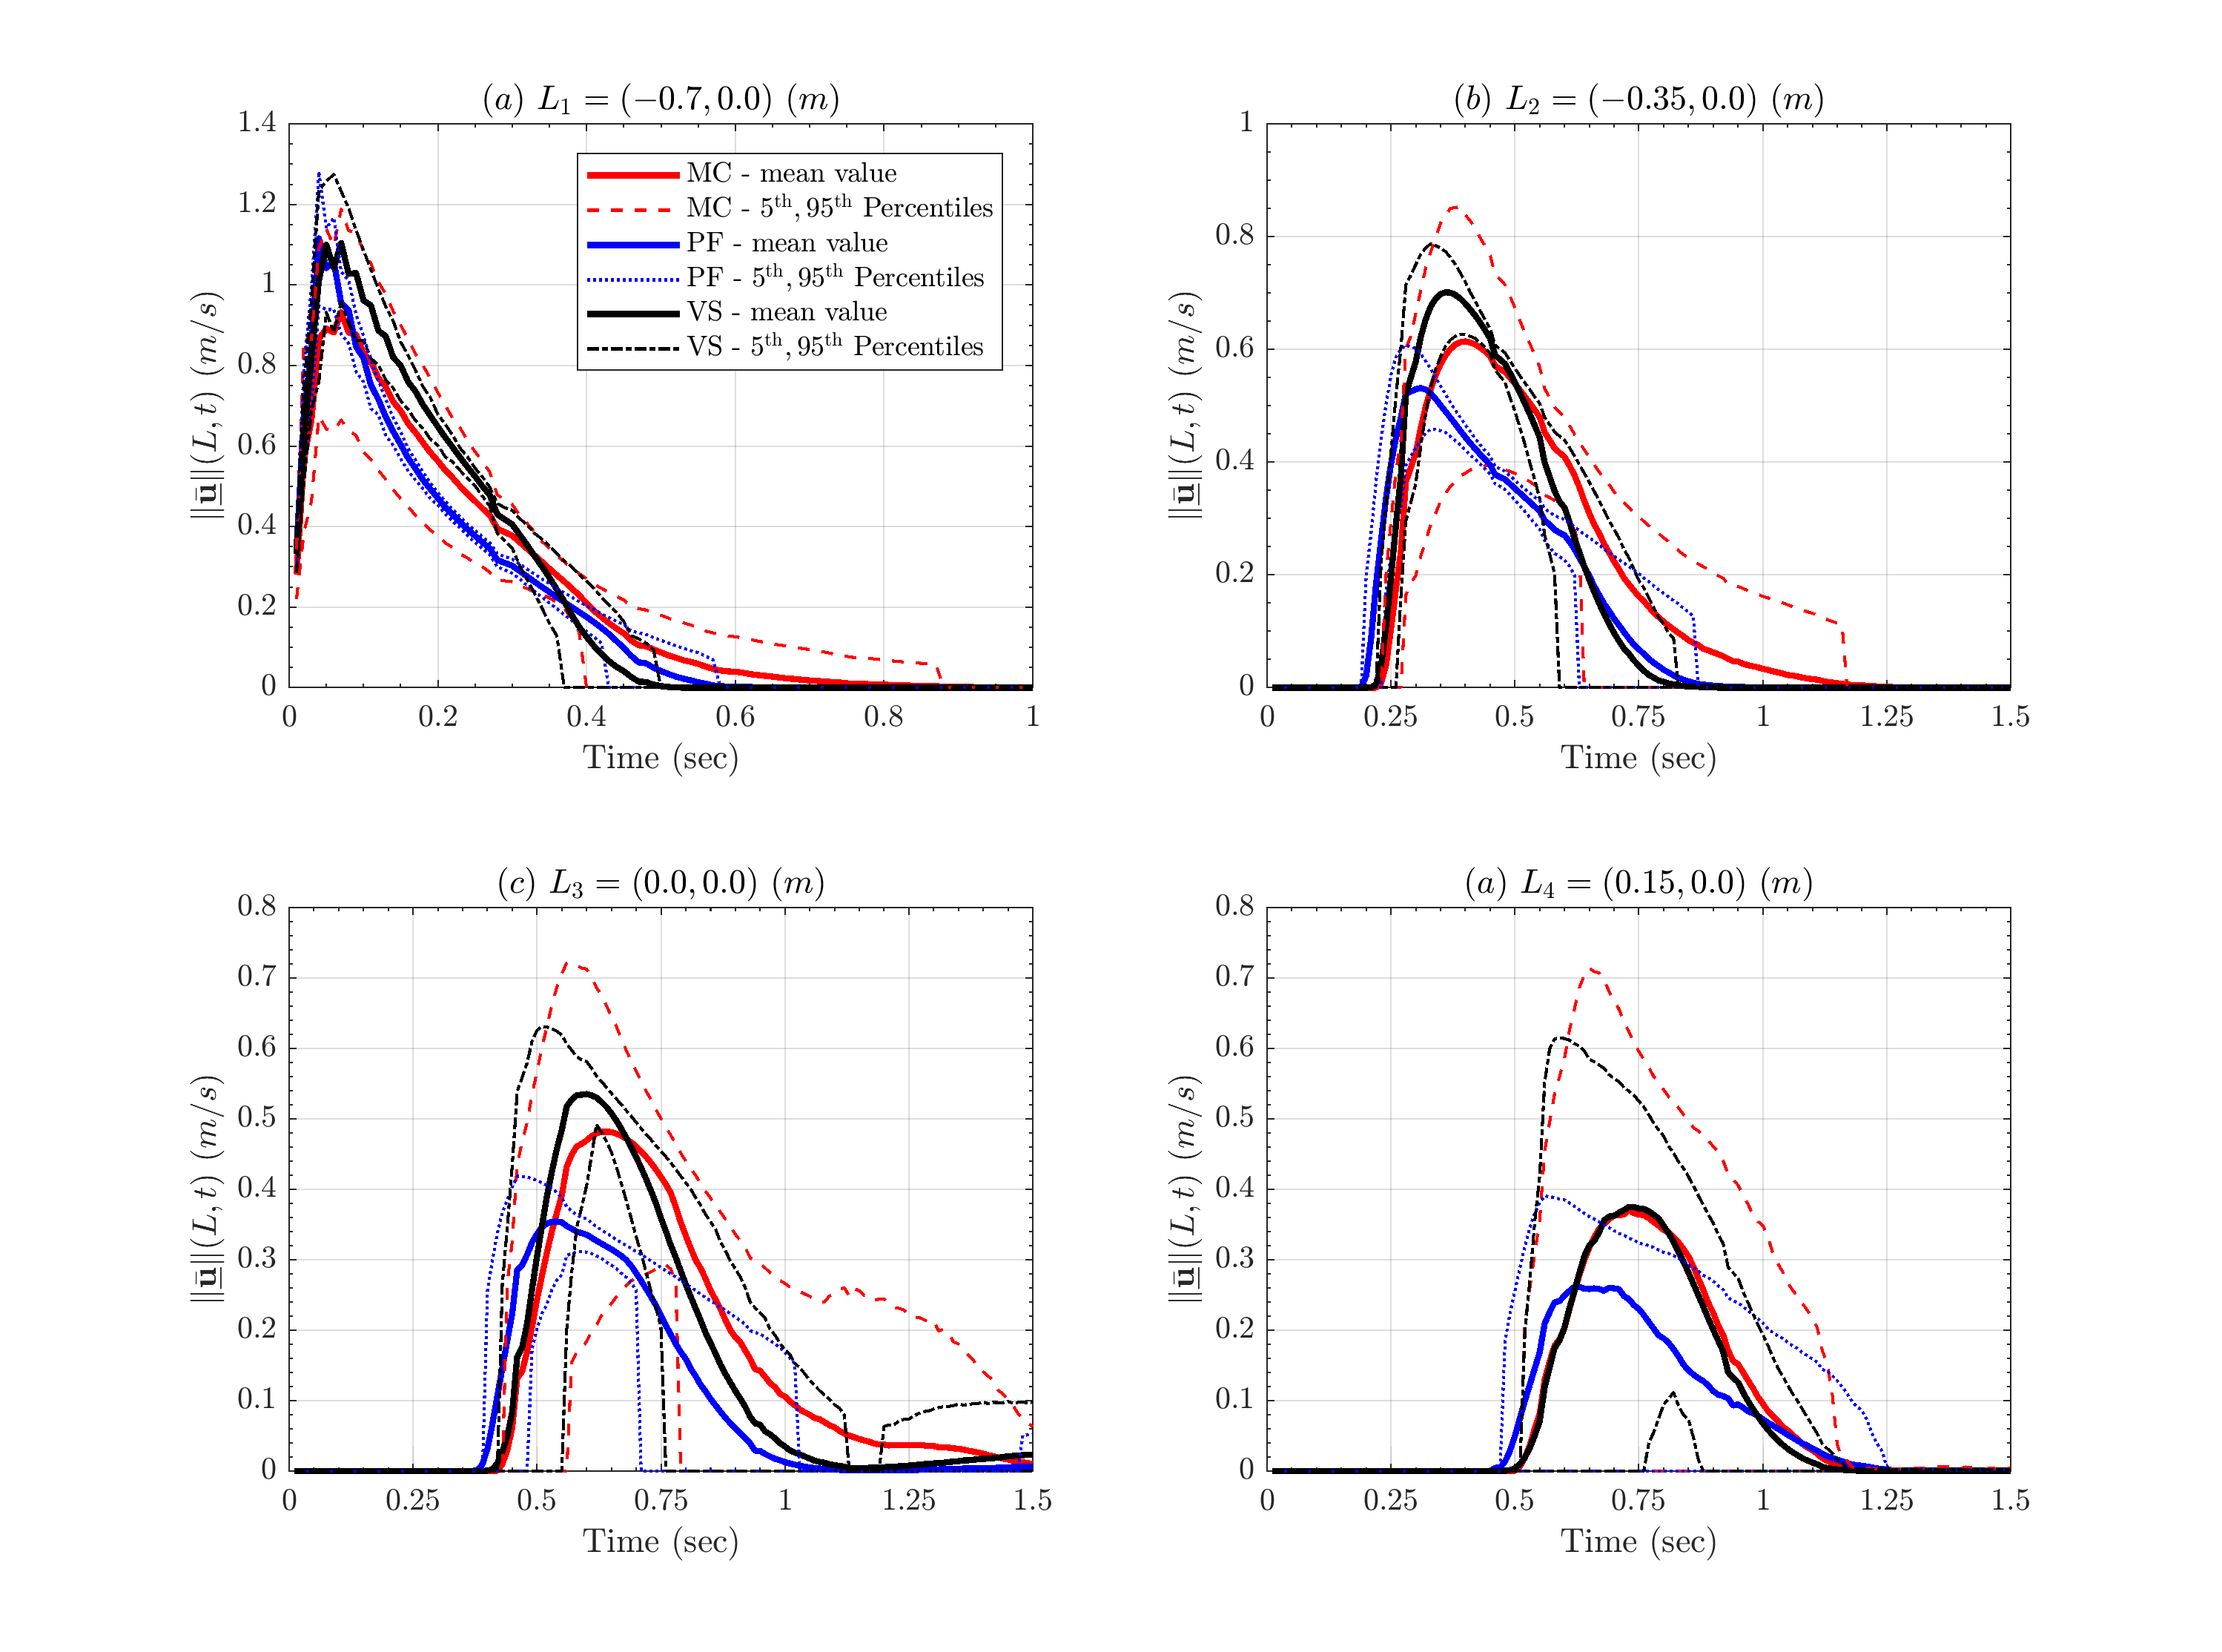
\includegraphics[width=1\textwidth]{InclinedPlane/LocalMeasurments/Velocity_Inc.png}
        \caption{Records of flow speed at four spatial locations of interest. Bold line is mean value, dashed/dotted lines are 5$^{\mathrm{th}}$ and 95$^{\mathrm{th}}$ percentile bounds. Different rheology models are displayed with different colors. Plots are at different scale.}
        \label{fig:Ramp-Vel}
\end{figure}
In plot \ref{fig:Ramp-Vel}a related to point $L_1$ speed peaks are $0.95 \pm 0.3$ m/s in MC, $1.1 \pm 0.2$ m/s in VS and PF. VS speed decreases almost linearly, while MC and PF have a more concave profile, making MC the faster model after $0.3$ sec. Plot \ref{fig:Ramp-Vel}b, related to point $L_2$, the peaks are $0.65 \pm 0.2$ m/s in MC, $0.7 \pm 0.1$ m/s in VS, and $0.52 \pm 0.08$ m/s in PF. In this case it is the PF model to decrease more linearly. In plot \ref{fig:Ramp-Vel}c, related to point $L_3$, peak velocity is $0.48$, $[+0.24, -0.20]$ m/s in MC, $0.54$, $[+0.1, -0.06]$ m/s in VS, and $0.36$, $[+0.06, -0.04]$ m/s in PF. In plot \ref{fig:Ramp-Vel}d, related to point $L_4$, peak velocity is $0.48$, $[+0.34, -0.48]$ m/s in MC, $0.48\pm 0.24$ m/s in VS, and $0.26$, $[+0.12, -0.26]$ m/s in PF. In all cases UQ shows that MC model uncertainty is remarkably larger than in the other models, and produces higher values in the 95$^{\mathrm{th}}$ percentile plots. Lowest speed values are affected by the elimination of material below $1$ mm flow height threshold. After $0.05$ s, the PF velocity profile is always significantly lower than the other models, but it also decreases slower, and matches with the stopping times of them. Moreover, it is worth noting that, curiously, PF reaches the points earlier. Speed in the deposits is below $0.1$ m/s in $L_3$, negligible in $L_4$.


\subsubsection{Forces terms}
Figure \ref{fig:Ramp-Fx-spatial} shows the spatial integral of the force terms in the slope direction, for the three rheology models. The spatial integration is performed on half spatial domain, due to the symmetry with respect to the flow central axis. In plot \ref{fig:Ramp-Fx-spatial}a $\boldsymbol{RHS_1}$ represents the effect of the gravity in all the models. It starts with a plateau at $\sim 1.3 N$ before $\sim 0.55 s$, then decreases to zero after the material crosses the change in slope. The force values are consistent with the expression $\rho \left(V/2\right) g_x$, representing half the weight of material, projected along the slope direction. Uncertainty range of $\pm 0.2 N$ on the peak values. MC decreases slower, and has a more significant uncertainty, after the change in slope. PF decreases faster. In plot \ref{fig:Ramp-Fx-spatial}b $\boldsymbol{RHS_2}$ represent the friction at the base of the flow. It is negative and opposed to the gravity. A similar profile is shared by the three models, with a first short-lasting weakening before $\sim 0.1 s$, a plateau with a small strengthening after $\sim 0.5 s$, and a final waning after $\sim 1 s$, at the conclusion of the dynamics. MC does not reach zero, while the other models do. VS values are generally $\sim 0.5 N$ weaker than MC, and PF is intermediate, except in the initial peak, where it is the weakest. Strongest forces are reached during the plateau, and are $\sim -0.55 N$, $\sim -0.75 N$, $\sim -0.9 N$, with uncertainty range of $\pm 0.25 N$ in the plateau. Uncertainty is reduced in the final stages of VS and PF, but increases in MC. In plot \ref{fig:Ramp-Fx-spatial}c $\boldsymbol{RHS_3}$ is related to the curvature effects, and is not null only at the change in slope. It is always negative, i.e. reducing flow velocity, indeed it is equivalent to the friction due to the additional weigh generated by centrifugal forces. Its scale is ten times smaller than the previous plots, with values above $0.1 N$ only in MC. VS displays a bimodal profile, with a second and weaker peak at $\sim 0.75 s$. In plot \ref{fig:Ramp-Fx-spatial}d $\boldsymbol{RHS_4}$ is related to the additional forces of the models, differently characterized. In MC and PF, they are significantly small forces before $0.1 s$, completely negligible later. In VS, this is the velocity dependent term. It is negative and plays a significant role. It reaches $\sim 1 N$ at the change in slope, with uncertainty $\pm 0.3 N$. It is bell shaped and null before $\sim 0.1 s$ and after $\sim 1 s$. In plot \ref{fig:Ramp-Fx-spatial}e $\sum^4_{i=1}\boldsymbol{RHS_i}$ represents the total force in the slope direction, and summarizes the previous plots. The profile is characterized by a positively valued stage at $\sim 0.5 N$ before the change in slope, and by a negatively valued stage after that, with bell-shaped profile, and a peak at $\sim -0.5 N$. In the first stage MC is more flat, while PF and VS decrease. In the second stage MC is occurring later in time, of $\sim 0.1 s$; PF and VS are remarkably similar, but VS wanes faster.
\begin{figure}[H]
        \centering
        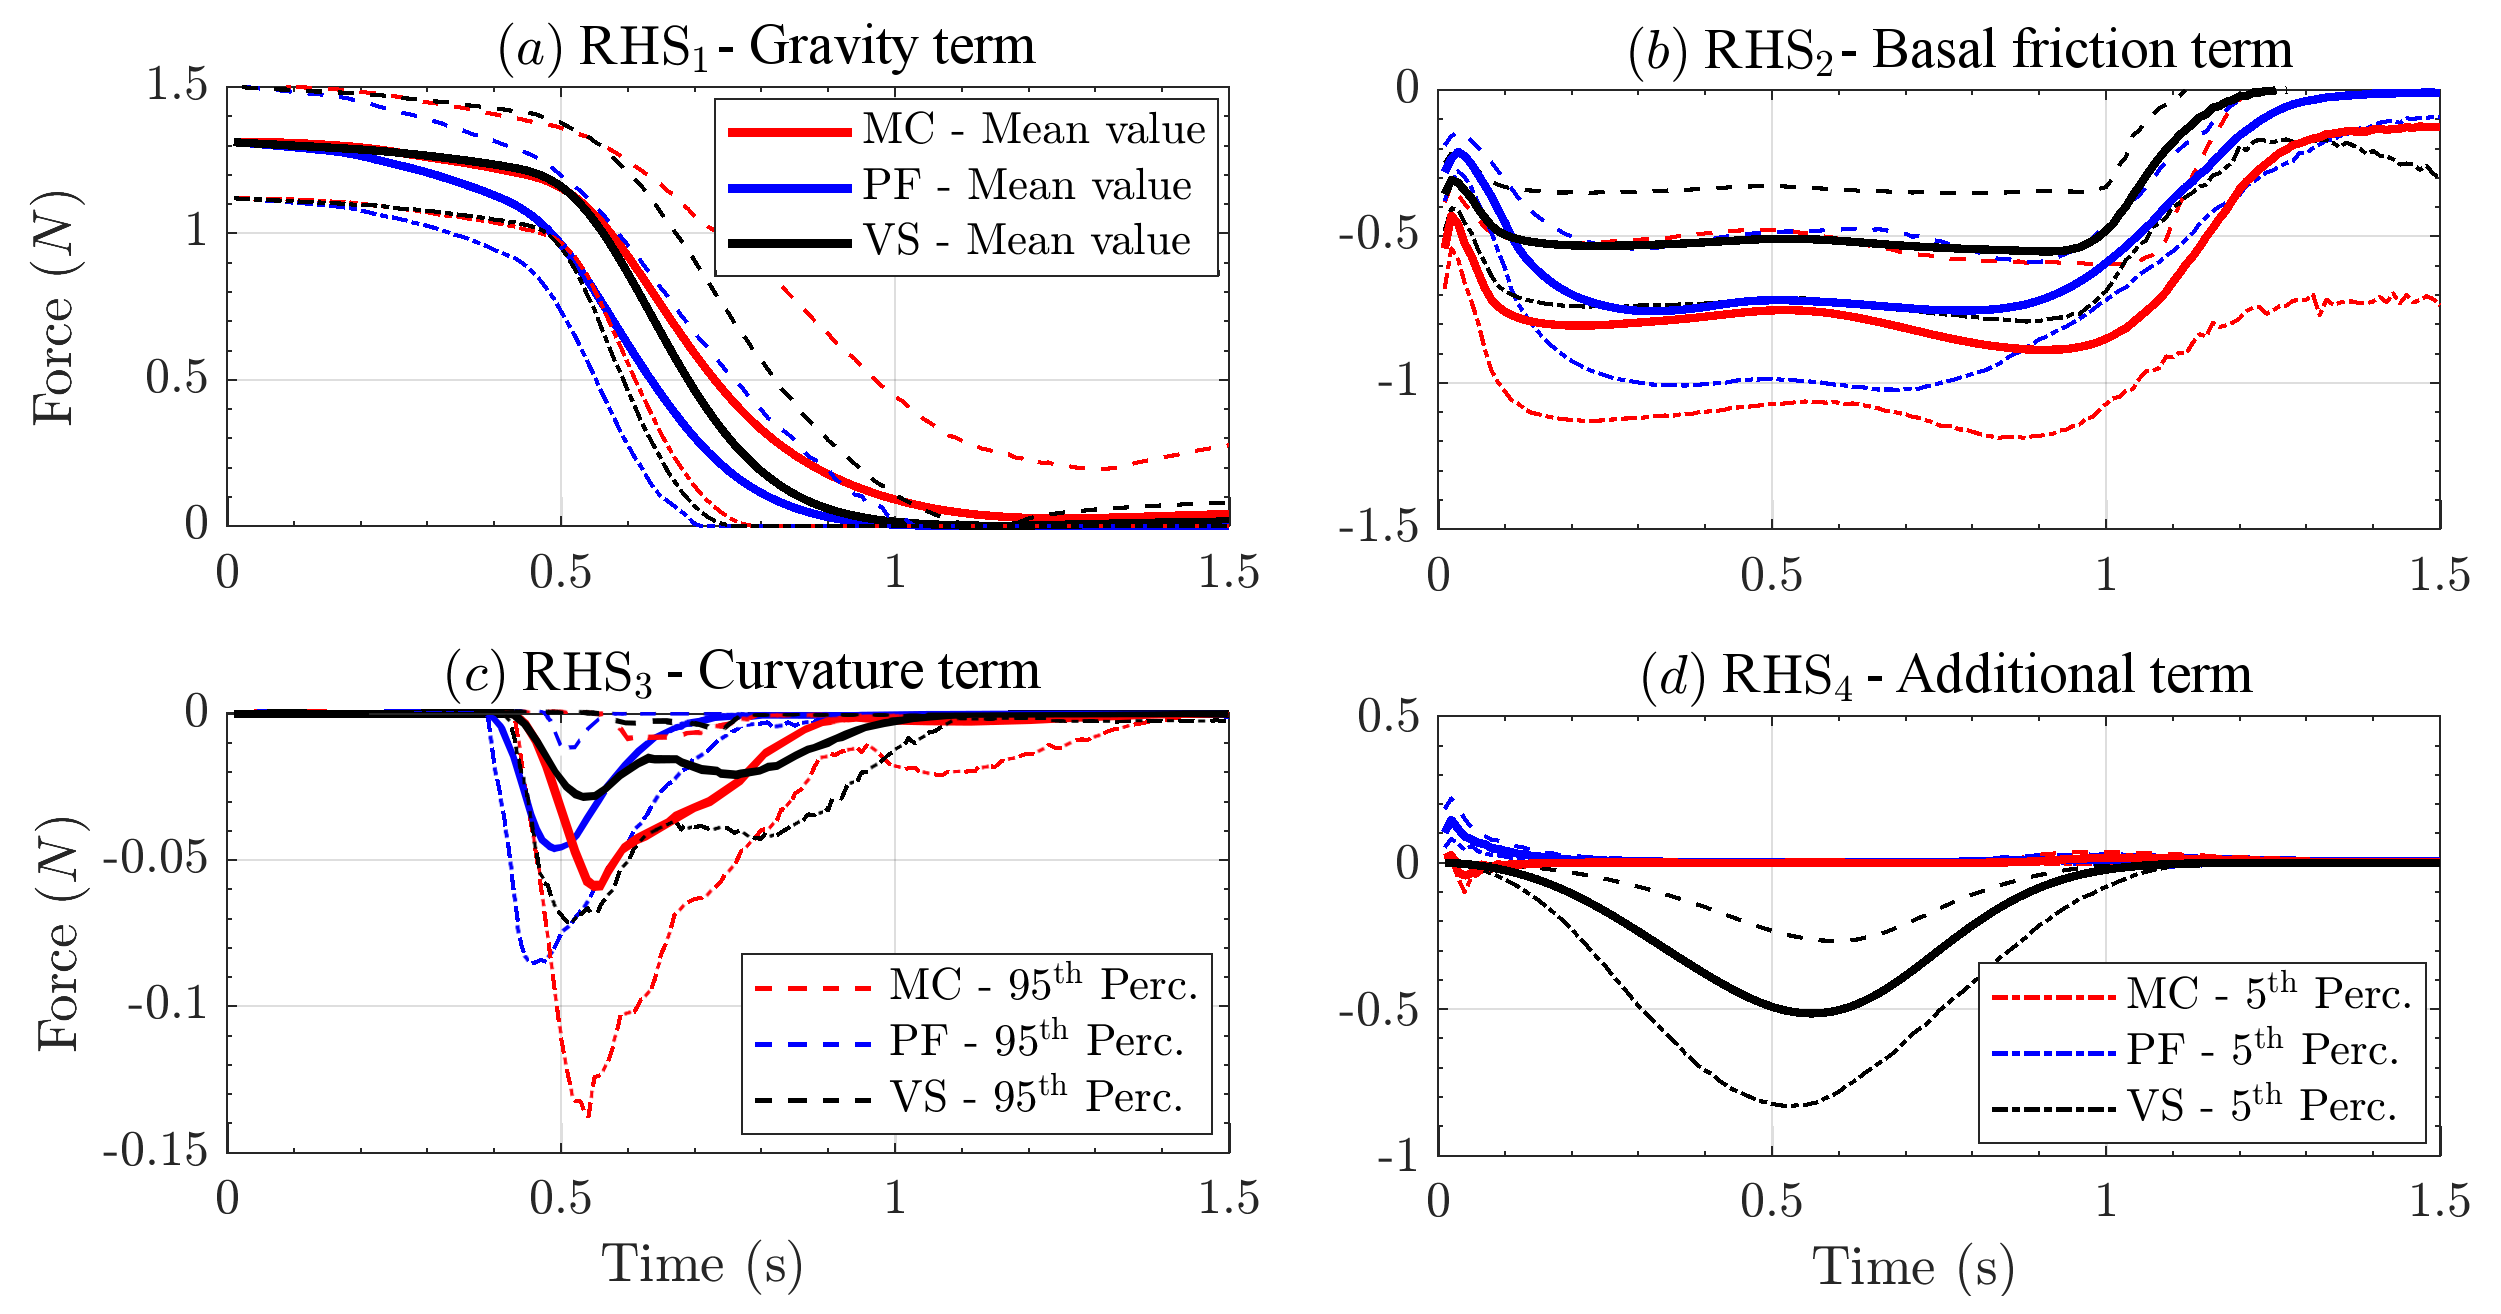
\includegraphics[width=1\textwidth]{InclinedPlane/AveragedMeasurments/ForcesIncline.png}
        \caption{Spatial sum of the RHS forces in the slope direction. Bold line is mean value, dashed lines are 5$^{\mathrm{th}}$ and 95$^{\mathrm{th}}$ percentile bounds. Scale of plot (c) is ten times larger than in (a),(b),(d); scale of plot (e) is slightly smaller.}
        \label{fig:Ramp-Fx-spatial}
\end{figure}


\subsubsection{Flow speed}
Figure \ref{fig:Colima-Vel} shows the flow speed, $\Vert \underline{\mathbf{u}} \Vert(L,t)$, at the points $(L_i)_{i=8,10,17,39,43,46}$, for the three rheology models. Like observed in Fig.\ref{fig:Colima-H}, pair of points $L_8$ and $L_{10}$, points $L_{17}$ and $L_{43}$, and points $L_{39}$ and $L_{46}$ have significantly similar plot profiles. In plot \ref{fig:Colima-Vel}a MC shows higher average speed, $\sim 80 m/s$, than PF and VS, both $\sim 70 m/s$. 95$^{th}$ percentile values can reach $150 m/s$ in MC, $140 m/s$ in VS, $130 m/s$ in PF. MC and PF are null after $20 s$, while VS decreases slower, and becomes null at $\sim 60 s$. In plot \ref{fig:Colima-Vel}b, the average peak values are $\sim 40 m/s$ in MC and PF, while only $20 m/s$ in VS. All the three models show 95$^{th}$ percentile values above $60 m/s$. VS speed decreases remarkably slower than in the other models, requiring more than $120 s$ to become null, while MC and PF speed remains positive for $\sim 25 s$. In plot \ref{fig:Colima-Vel}c, average speed is $\sim 20 m/s$ in PF, $\sim 10 m/s$ in MC, $\sim 2 m/s$ in VS. 95$^{th}$ percentile values can reach $\sim 55 m/s$ in PF, $\sim 48 m/s$ in MC, $\sim 24 m/s$ in VS. The duration of positive velocity in VS can be long hundredths of seconds. A very similar situation is pictured in plot \ref{fig:Colima-Vel}e. Instead in plot \ref{fig:Colima-Vel}d, only MC shows a max speed above $3 m/s$, the 95$^{th}$ percentile values at $\sim 15 m/s$. In the other models the average speed is always below $1 m/s$ and the 95$^{th}$ percentile values have an increasing profile followed by a slightly decreasing plateau, at $\sim 2 m/s$ in VS, $\sim 1 m/s$ in PF. VS can have a speed above $\sim 1 m/s$ at $\sim 3600 s$. In plot \ref{fig:Colima-Vel}f, only MC shows an average speed above zero, while in the other models even the 95$^{th}$ percentile values are always below $\sim 0.5 m/s$, and start to be positive only at $\sim 200 s$ in PF, and $\sim 600 s$ in VS. MC can have speed at $\sim 1 m/s$ for more than $\sim 500 s$, but the plot is very noisy.
\begin{figure}[H]
         \centering
        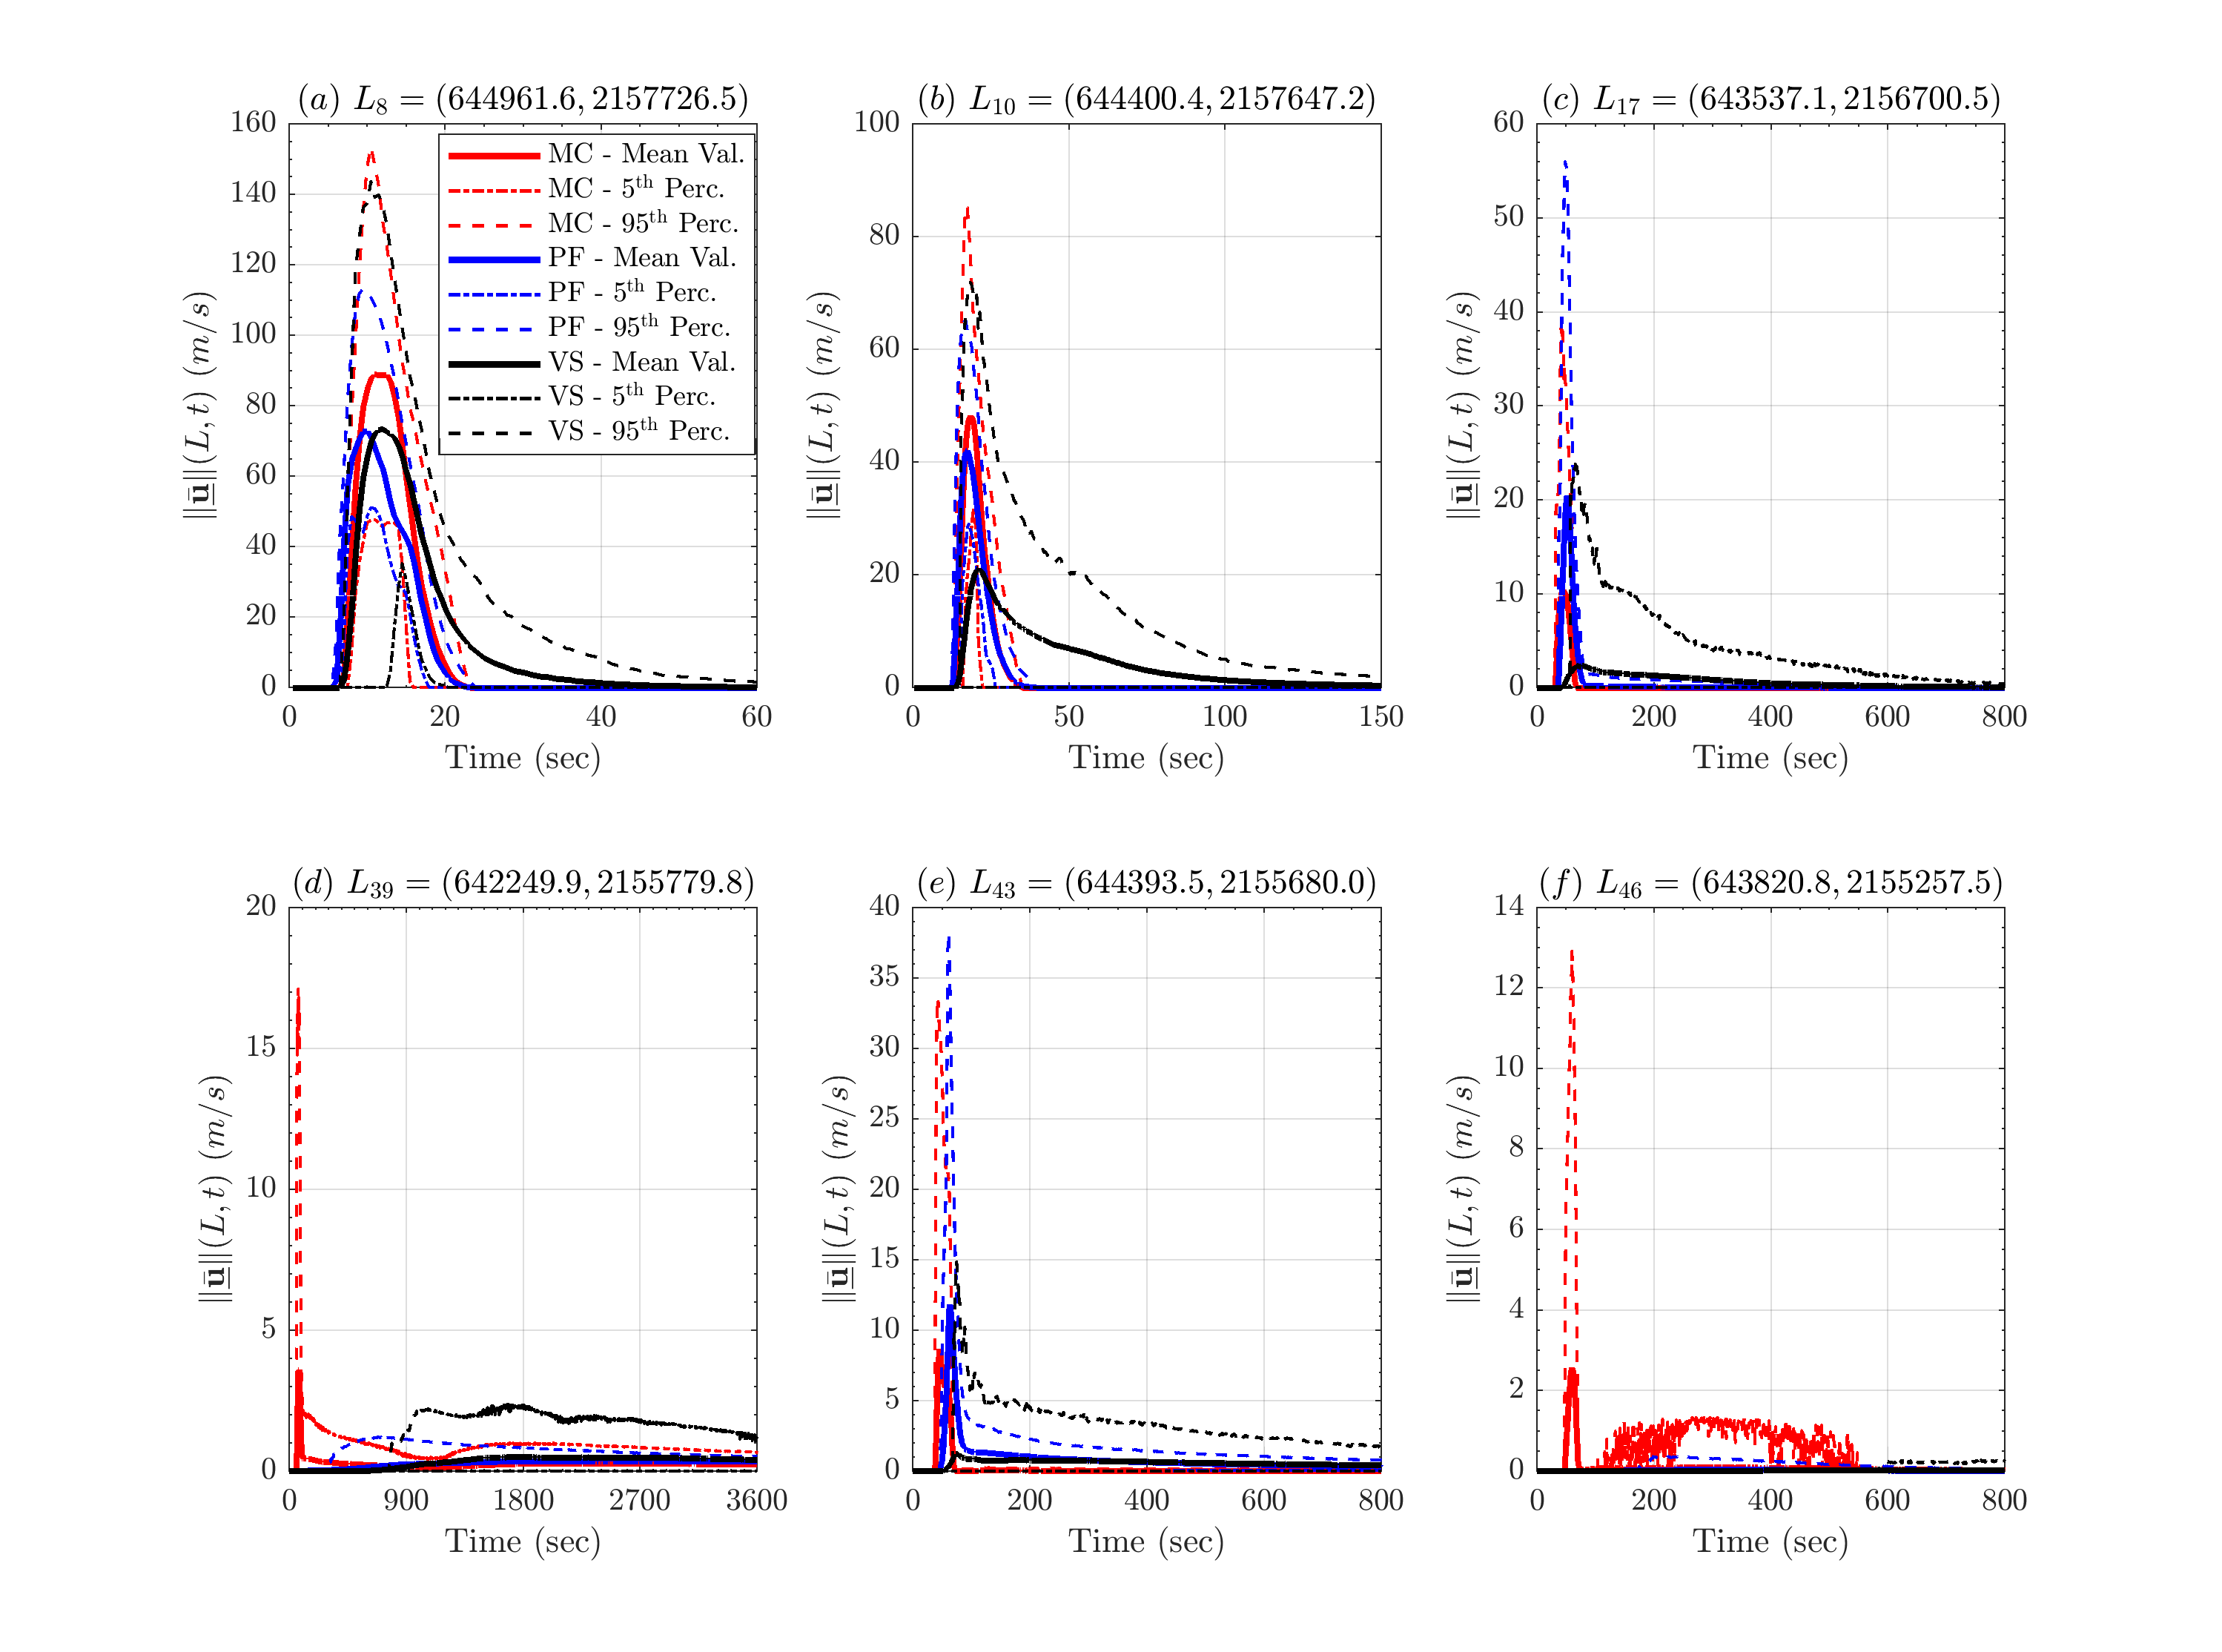
\includegraphics[width=1\textwidth]{BAF_VolcanDeColima/LocalMeasurments/Velocity_Col.png}
        \caption{Records of flow speed at six selected locations. Bold line is mean value, dashed/dotted lines are 5$^{\mathrm{th}}$ and 95$^{\mathrm{th}}$ percentile bounds. Different rheology models are displayed with different colors. Plots are at different scale. Numerical noise affecting percentile curves in (f) has been averaged.}
        \label{fig:Colima-Vel}
\end{figure}


\subsubsection{Flow speed}
Figure \ref{fig:BAF-V-MC} shows the mean flow speed, $h(L,t)$, at the 51 spatial locations of interest, according to MC.
\begin{figure}[H]
         \centering
        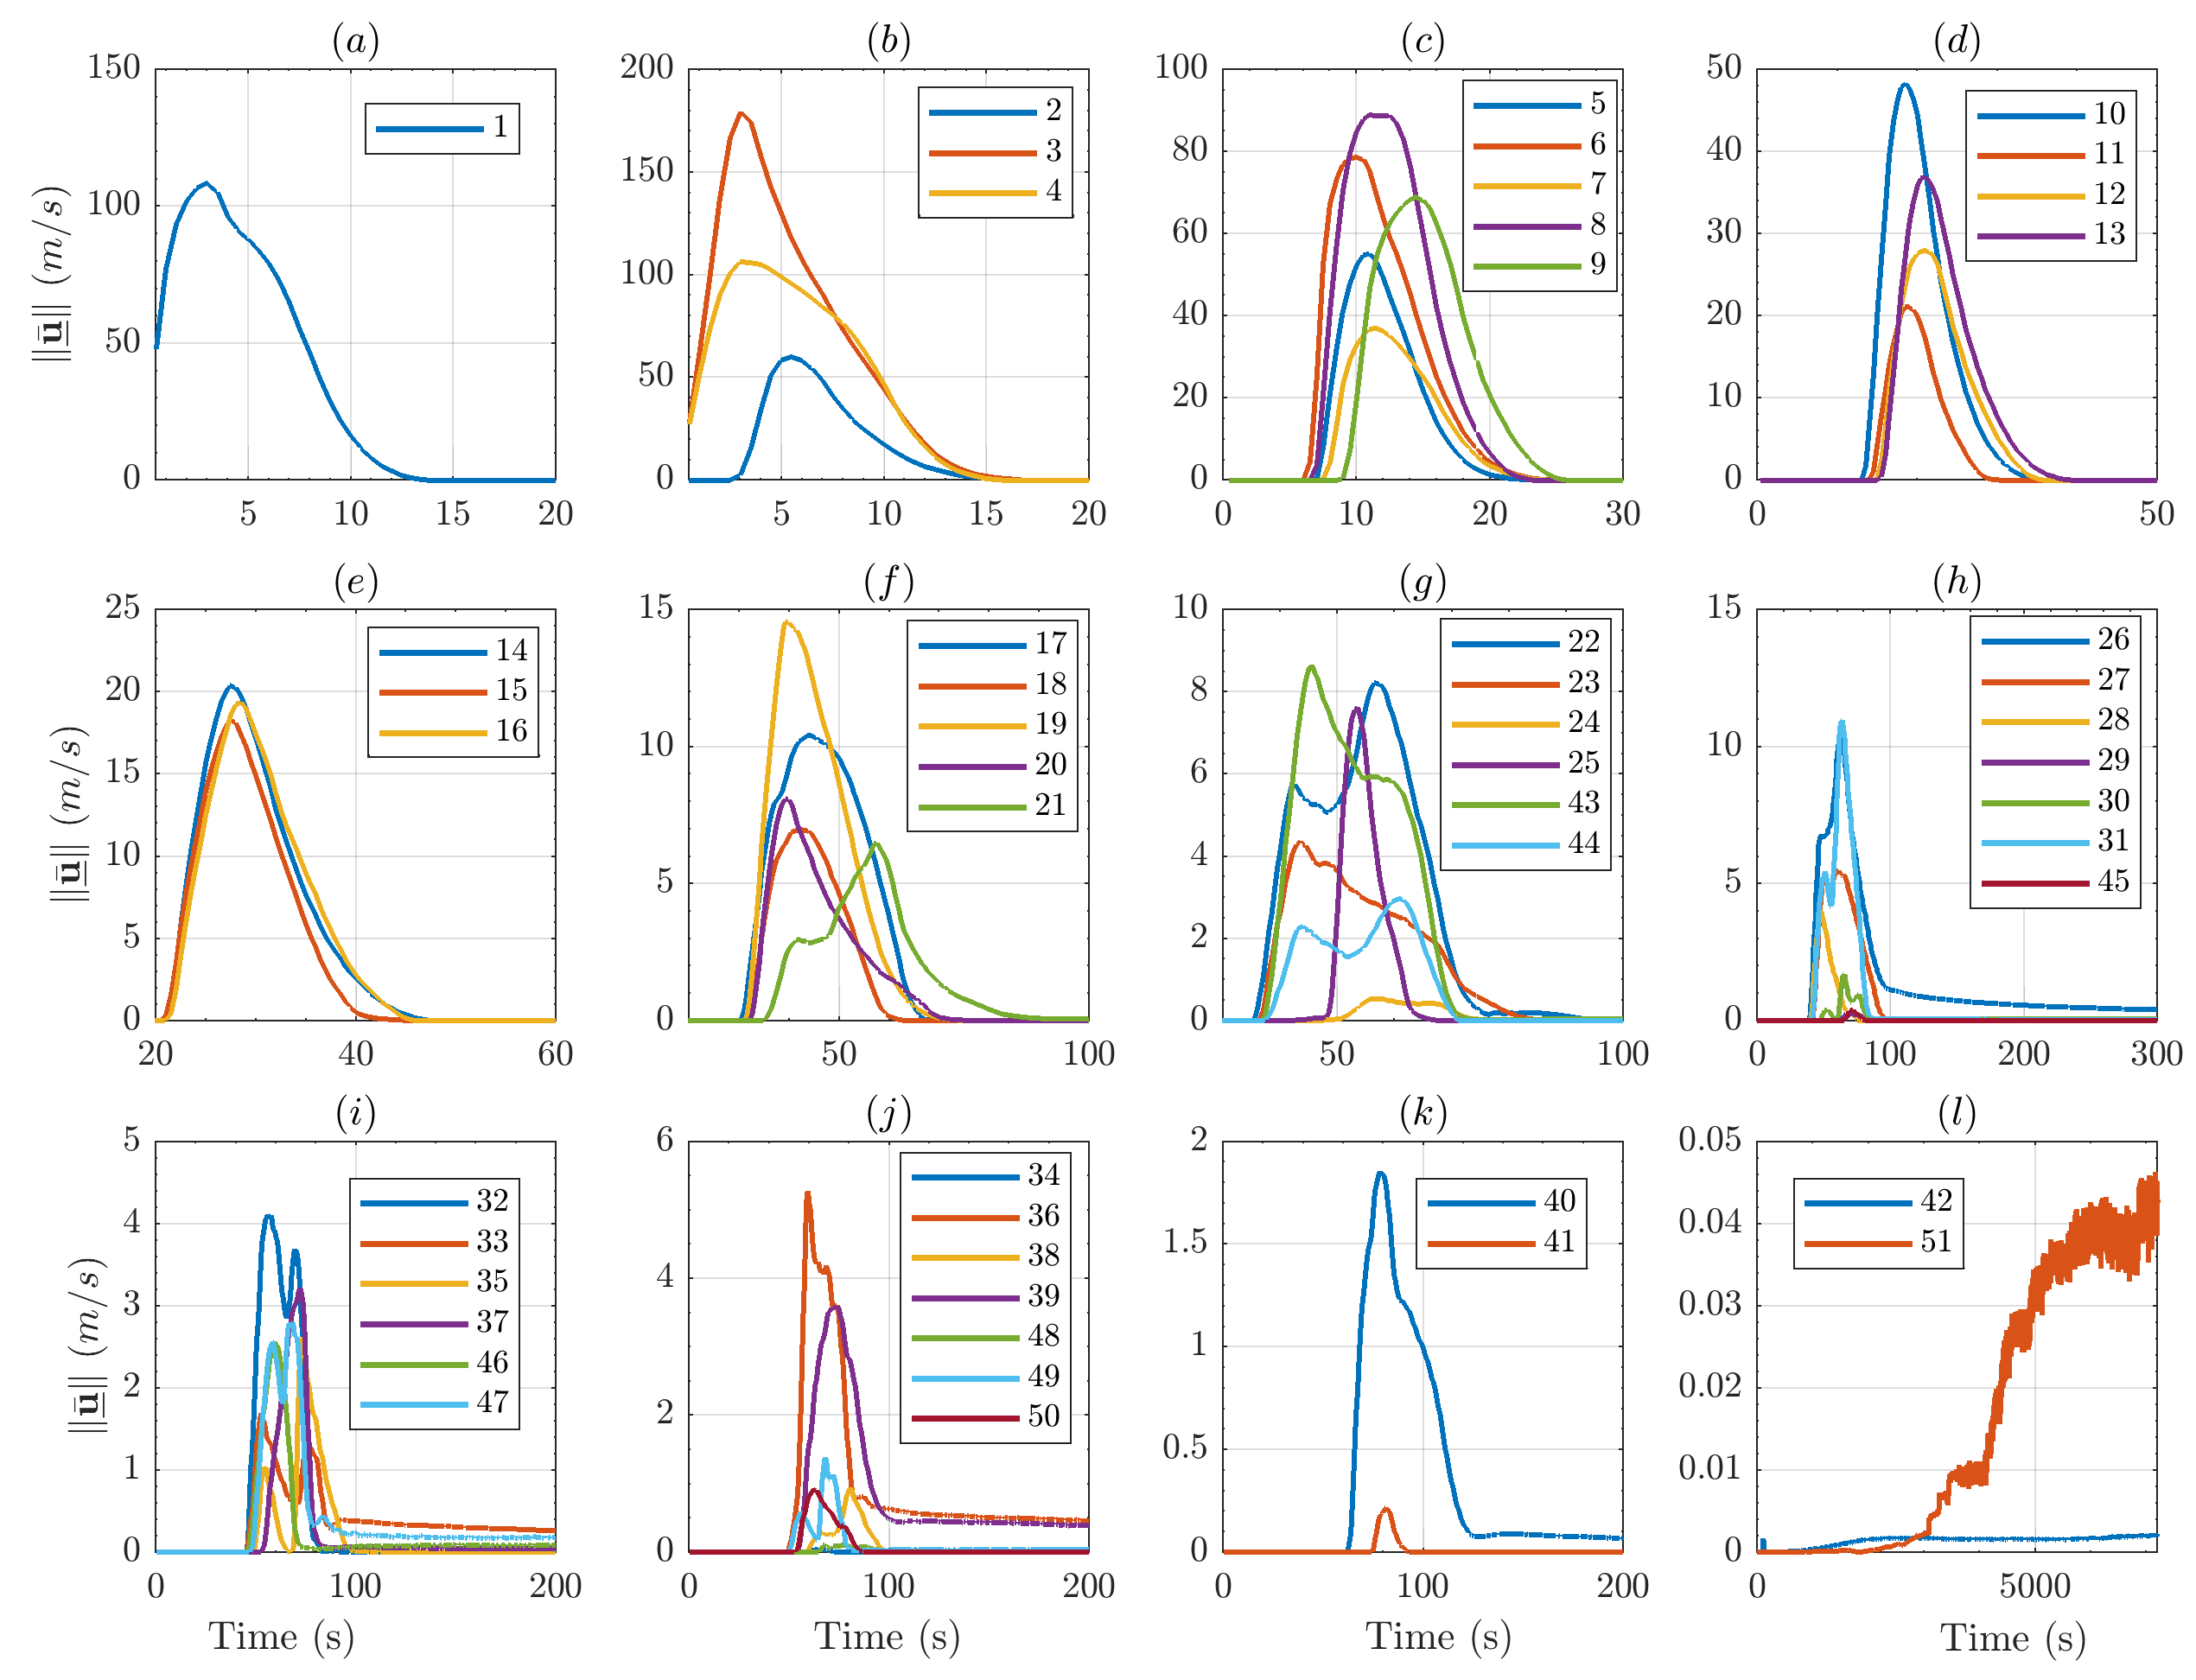
\includegraphics[width=1\textwidth]{MC&VS_51/Velocity_MC3.png}
        \caption{MC model, records of average flow speed, $\vert\underline{u}\vert(L,t)$, in 51 spatial locations of interest (Fig. \ref{fig:Colima-first}).}
        \label{fig:BAF-V-MC}
\end{figure}
Again the different plots have different scales on either time and space axes. The plot profiles are similar to what observed in figure \ref{fig:Ramp-Vel}, following the plot profile classification described above. Maximum speed of $\sim 200 m/s$ is observed in proximity of the initial pile, in plot \ref{fig:BAF-V-MC}b, and it is related to the initiation collapse dynamics. After 1 km runout (horizontal projection), in plot \ref{fig:BAF-V-MC}e, the max speed is ten times smaller, $\sim 20 m/s$. At about 2 km from the initiation, when entering the main ravines, speed is $\sim 10 m/s$, and becomes $\sim 5 m/s$ or less in the distal part of the ravines.  In detail, in plots  \ref{fig:BAF-V-MC}f,g,h,i,j, the speed often shows bimodal profiles, not observed in the inclined plane case study. Moreover, in plots \ref{fig:BAF-V-MC}h,i,j, positive asymptotes are sometimes observed, meaning a slowly and steadily moving material even minutes after the collapse.


\subsubsection{Force terms}
Figure \ref{fig:Colima-F-spatial} shows the spatial sum of the force terms moduli, for the three rheology models.
\begin{figure}[H]
        \centering
        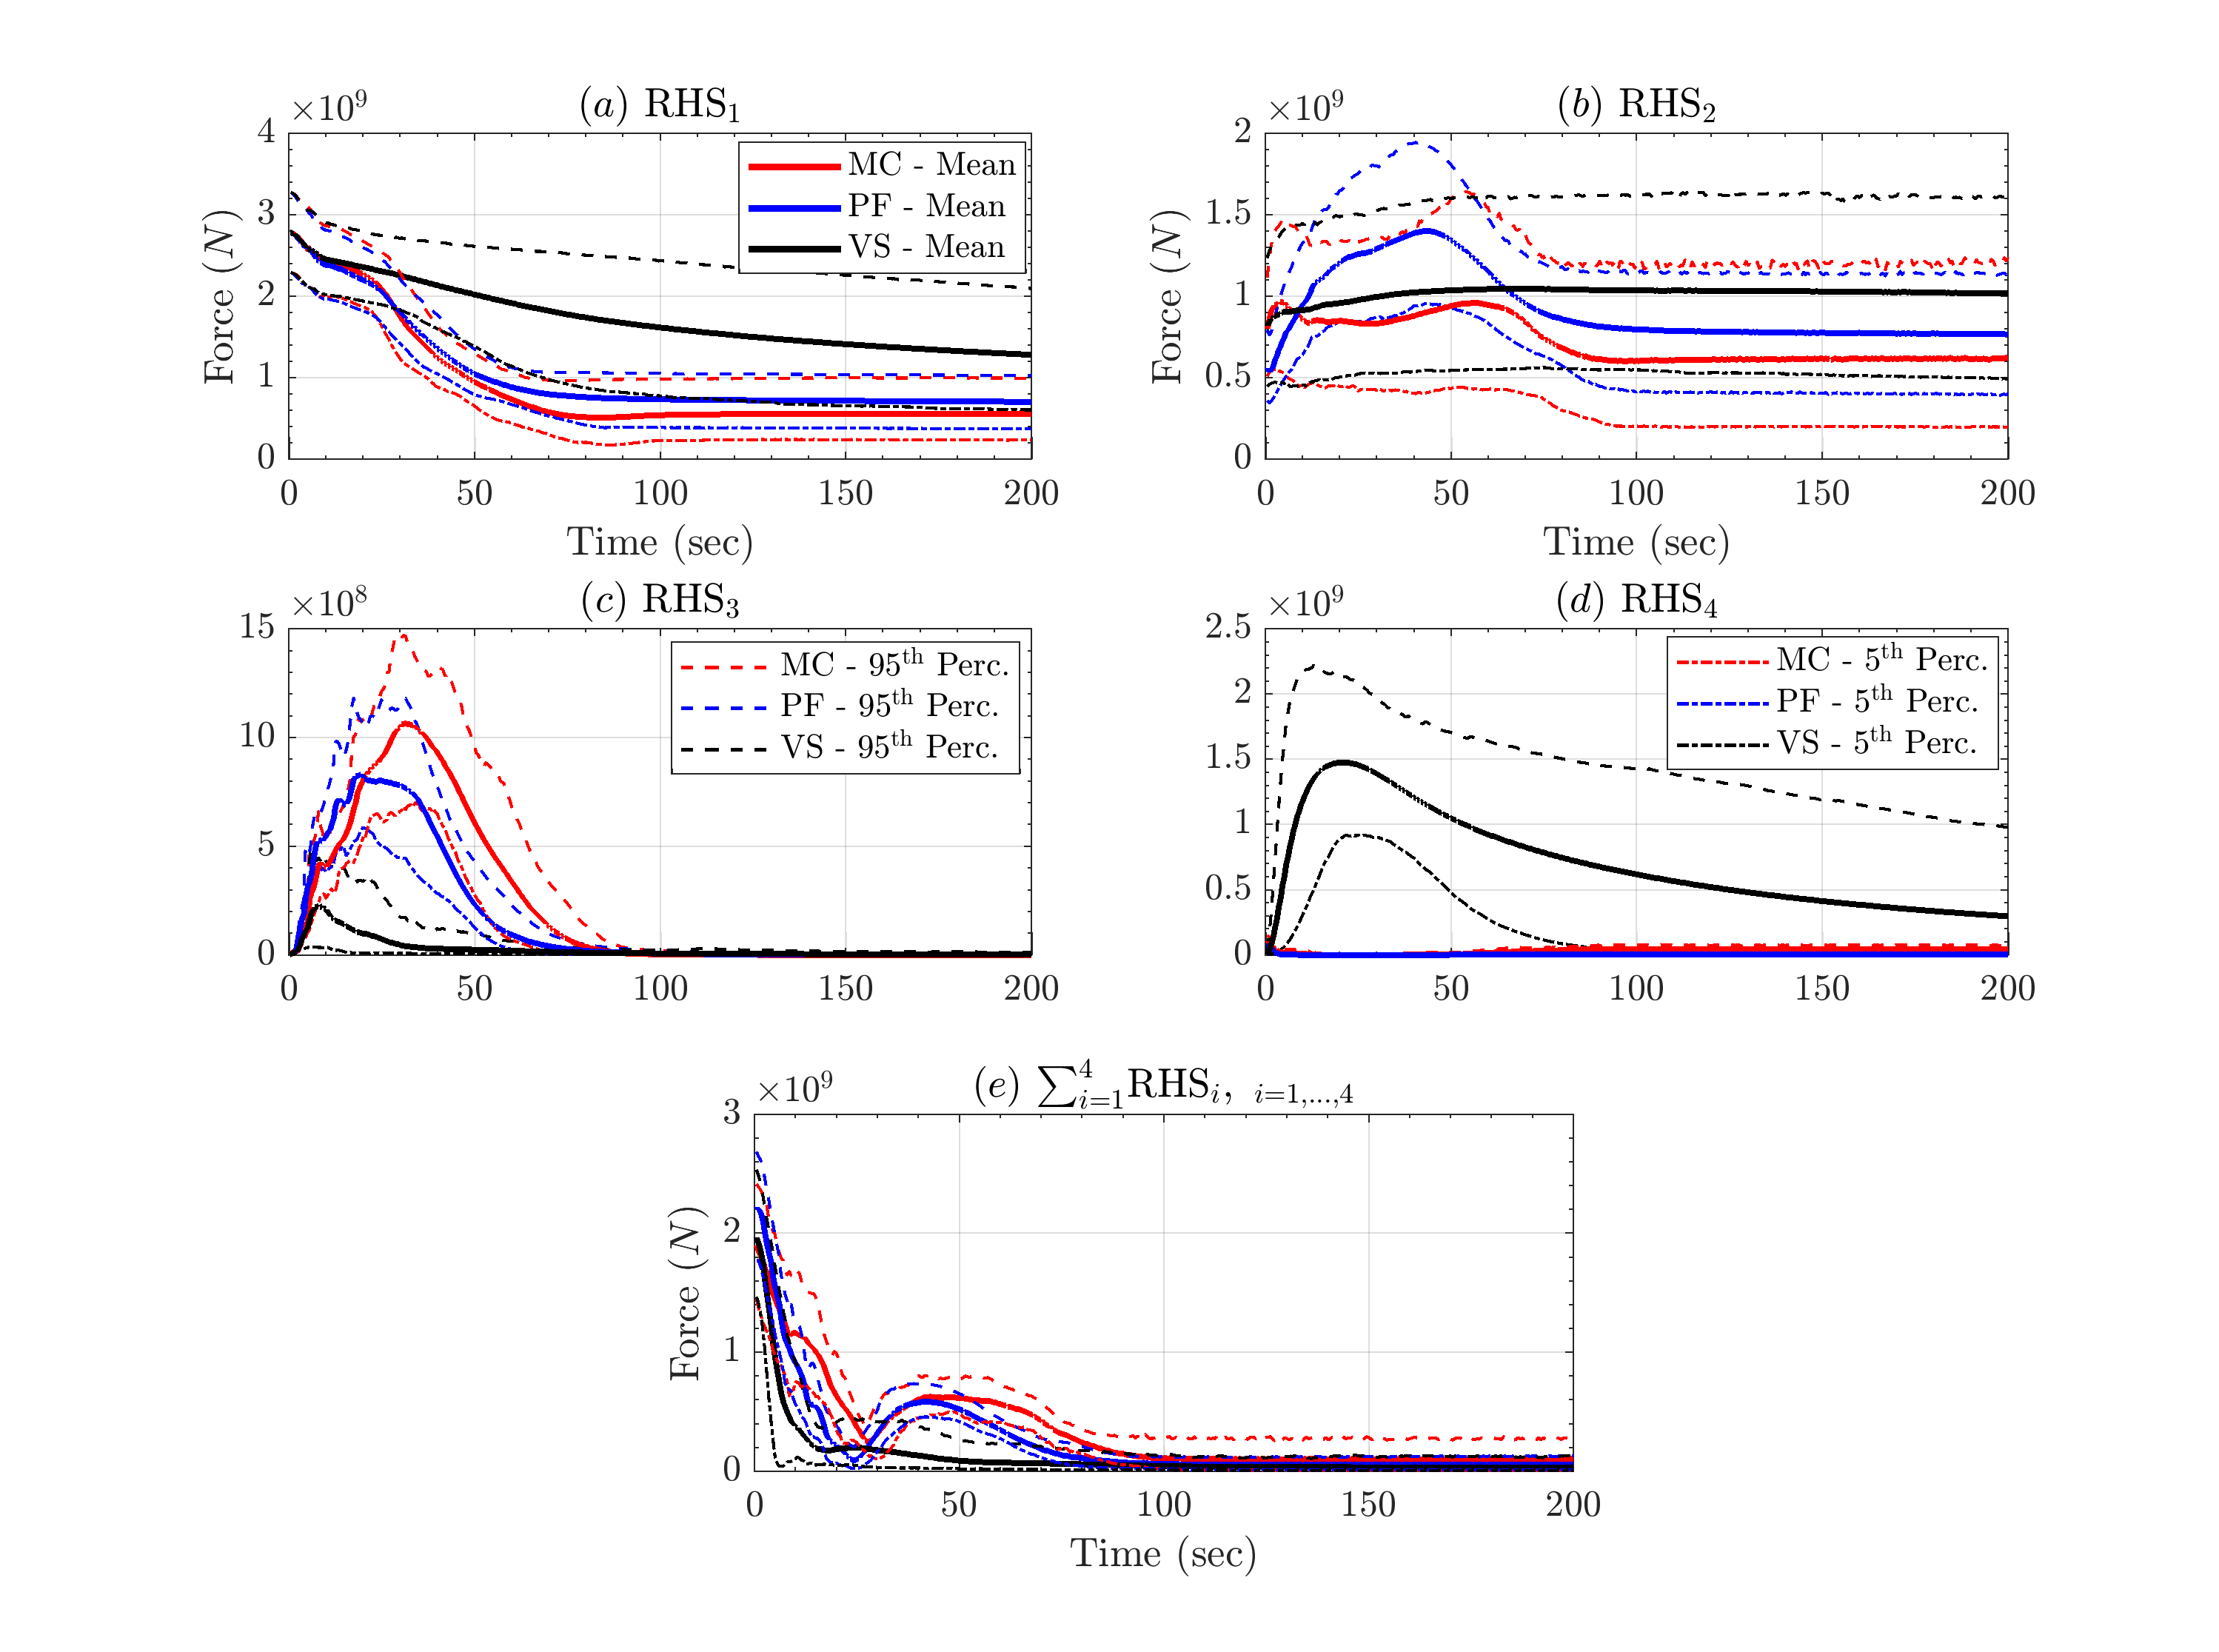
\includegraphics[width=1\textwidth]{BAF_VolcanDeColima/AveragedMeasurments/ForcesColima.png}
        \caption{Spatial sum of the RHS force terms moduli. Bold line is mean value, dashed lines are 5$^{\mathrm{th}}$ and 95$^{\mathrm{th}}$ percentile bounds.}
        \label{fig:Colima-F-spatial}
\end{figure}
The figure can be compared with Fig. \ref{fig:Ramp-Fx-spatial}, which was related to forces in the slope direction in the inclined plane case study. In plot \ref{fig:Colima-F-spatial}a $\boldsymbol{RHS_1}$ represents the effect of the gravity in all the models. It is decreasing in all the models, but more gradually in VS than in the others. Initial values are $2.8e9 N$ in all the models, uncertainty $\pm 2.5e8 N$. Force values are consistent with the material weight component along the mountain slope, and their decrease is related to the slope reduction. At $\sim 10 s$ all the models show a slowing down of the decrease, which is permanent in VS, and lasting $10 s$ in MC and PF. The latter models, reach a flat profile after $\sim 60 s$, at $6e8 N$ and $7e8 N$, respectively, and uncertainty of $\pm 2e8 N$ and $1.5e8 N$. VS, which flattens more gradually, is $1.3e9 N$ at $200 s$, uncertainty $[-7e8,+8e8] N$. In plot  \ref{fig:Colima-F-spatial}b $\boldsymbol{RHS_2}$ represents the effect of the basal friction in all the models. In MC, shows a bimodal profile, with a peak at $5 s$, and a second one at $60 s$. Both of them at $9.5e8 N$ on average, with uncertainty of $[-4e8,+5e8] N$ in the first peak, and $[-5e8,+7e8] N$ in the second. The minimum between the two peaks is at $8e8 N$ and lasts from $10 s$ to $30 s$. After the second peak there is significant decrease, reaching $6e8 N$ at $90 s$, and becoming flat. Final uncertainty is $[-4e8, +6e8] N$. In PF, the plot starts from lower initial values than in the other models, but then has a unimodal peak of $1.4e9 N$ at $40 s$, on average. Uncertainty $\pm 5e8 N$. After that, the plot decreases, reaching $7.5e8 N$ at $90 s$, and becoming flat. Final uncertainty is $\pm 3.5e8 N N$, lower than in the other models. In VS, there is slow increase until the plot reaches $1.05e9 N$ at $70 s$. Then the average force is almost flat, at $1.0e9 N$, with significant uncertainty of $[-5e8,+6e8] N$. In plot \ref{fig:Colima-F-spatial}c $\boldsymbol{RHS_3}$ represents the effect of the curvature of terrain. The three models all show a bell-shaped profile, waning to zero at $90 s$. However, MC has reaches $1.1e9 N$ at $30 s$, PF $8e8 N$ at $20 s$, VS $2.5e8 N$ at $10 s$. The rise has a similar profile, but a different duration. The decrease is more gradual in VS. Uncertainty at the peak value is $\pm 4.5e8 N$ in MC, $[-2.5e8,+3.5e8] N$ in PF, $\pm 2e8 N$ in VS. In plot \ref{fig:Colima-F-spatial}d $\boldsymbol{RHS_4}$ has a different meaning in the three models. In MC it is the internal friction term, and it has a small peak in the first second, at $1e8 N$. After that it flattens to negligible values, but shows again values at $5e7 N$ after $60 s$. In PF it is the a depth averaged correction in the hydrostatic pressure, and has a almost negligible effect only in the first second, at $5e7 N$. In VS, instead, it is the velocity dependent term, and has a very relevant effect. The plot shows a bell-shaped profile, with a peak of $1.45e9 N$ at $20 s$. Uncertainty is $[-5.5e8, +6.6e8] N$, at the peak. After that, the force gradually decreases, and is $3e8 N$ at $200 s$, on average. Uncertainty $[-3e8, +7e8] N$. In plot \ref{fig:Colima-F-spatial}e, the modulus of the total force $\sum^4_{i=1}\boldsymbol{RHS_i}$ is shown, with the complex interplay between the terms. First a steep decrease due to the domination of the gravity upon the friction, then a bell-shaped increase when the friction stops the dynamics.


\subsubsection{Flow speed}
Flow speed enriches our analysis of additional details. In Fig. \ref{fig:Ramp-Vel} MC has a fatter tail, due to the already observed distal spreading of material. PF profile is more concave at the beginning, due to the combined effects of the dual bed friction angle and the hydrostatic correction. In Fig. \ref{fig:Colima-Vel} VS is confirmed to be significantly slower than the other models, after the initial collapse. Moreover, it is the only model which presents slowly moving material for all the simulation, near the initiation pile. MC shows short lasting peaks of speed even in the most distal sample points, due to the lack of a strong slowing mechanism like the secondary angle in PF, and the speed dependent term in VS.  





\newpage
\paragraph{Example 1 - Flow down and inclined plane}
Figure \ref{fig:Ramp-Ci_x} shows the Contributions Coefficients $(C_i)_{i=1,\dots,4}$, for the three rheology models and focusing on the RHS terms in the slope direction. The different models are plotted separately: \ref{fig:Ramp-Ci_x}a,d,g,j assume MC; \ref{fig:Ramp-Ci_x}b,e,h,k assume PF; \ref{fig:Ramp-Ci_x}c,f,i,l assume VS.
\begin{figure}[H]
         \centering
        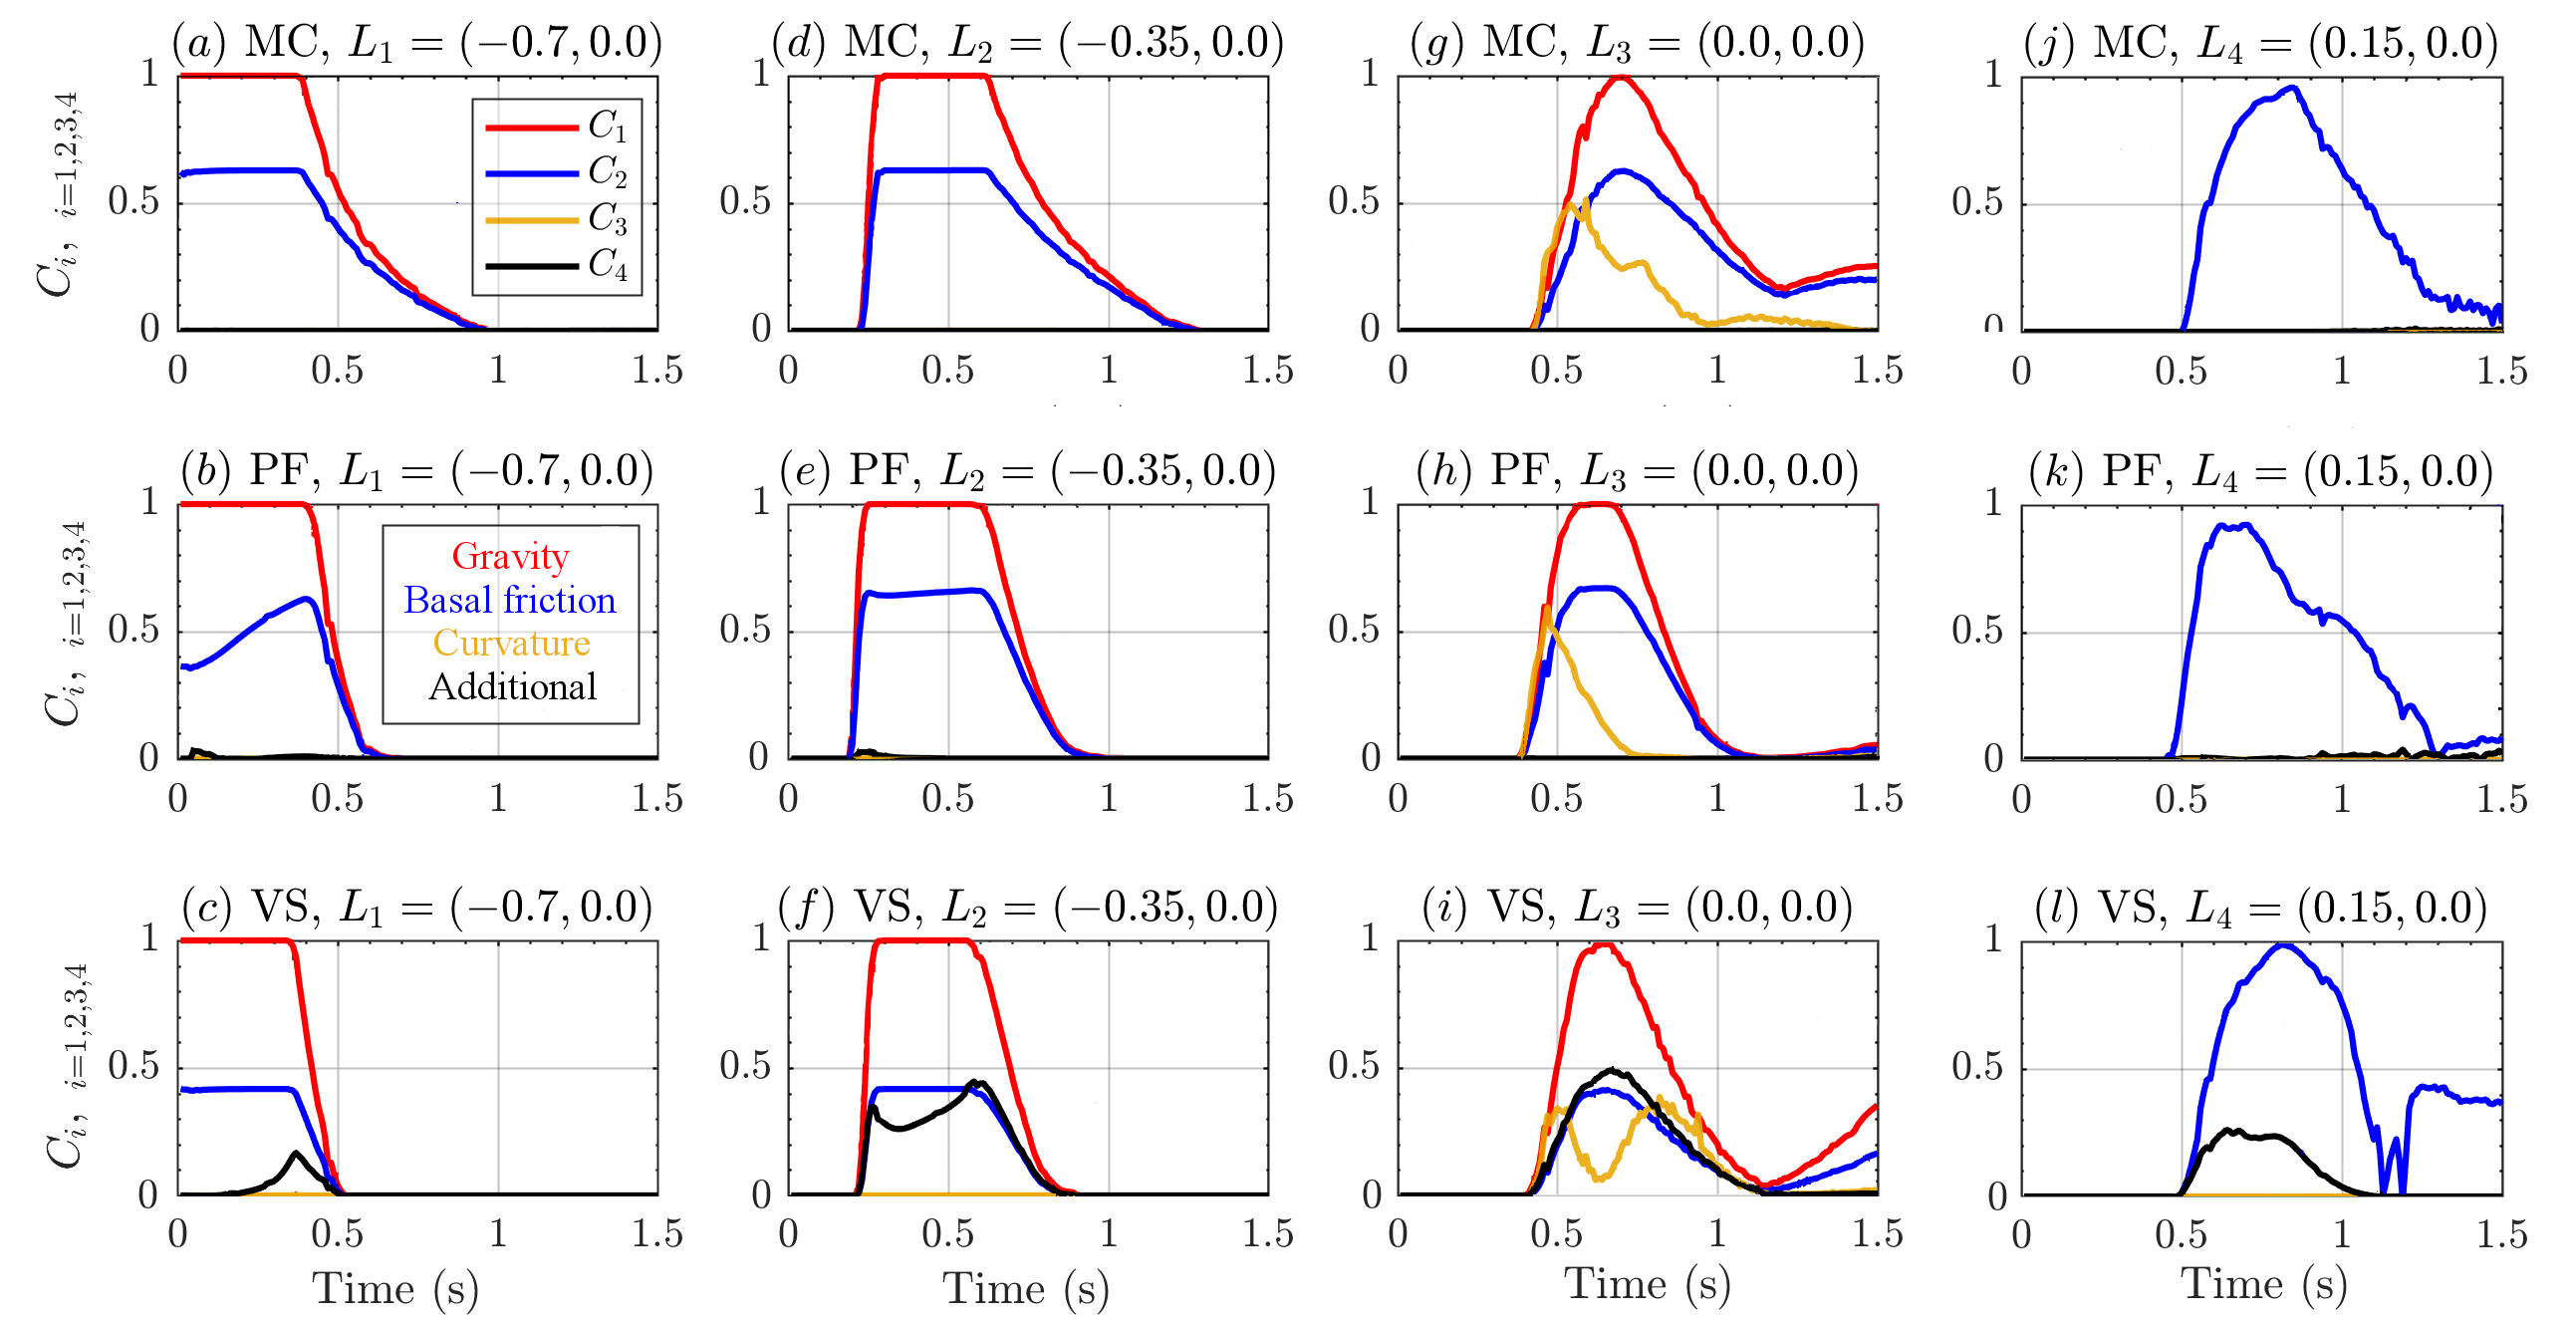
\includegraphics[width=1\textwidth]{InclinedPlane/ForceContrib/Ci_x.png}
        \caption{Records of contribution coefficients of \textbf{RHS} forces, in the slope direction, in four spatial locations of interest. Different rheology models are displayed with different colors. Dominant function $\Phi$ is calculated based on the $l^\infty$ norm}
        \label{fig:Ramp-Ci_x}
\end{figure}
The plots \ref{fig:Ramp-Ci_x}a,b,c are related to point $L_1$, placed on the initial pile. $C_1$ and $C_2$ play the major roles, with a minor contribution $C_4$ in VS. Contributions profiles are flat plateaus that start to wane after $0.4 s$, with the rise of the probability of no-flow at the point $L_1$ (see also Fig. \ref{fig:Ramp-Pr_x}. Uncertainty is related to the no-flow times, and to the value of $C_2$. The contribution $C_4$ can be significant, as it is shown by the 95$^{\mathrm{th}}$ percentile values, but appears after $0.25 s$. The plots \ref{fig:Ramp-Ci_x}d,e,f are related to point $L_2$, placed in the middle of the slope. Again the major contributions are $C_1$ and $C_2$, with trapezoidal profile preceded and followed by no-flow. In VS, $C_4$ becomes as a significant as $C_2$, but it is bimodal instead than trapezoidal. The plots \ref{fig:Ramp-Ci_x}g,h,i are related to point $L_3$, placed at the change in slope. The contributions $C_1$ and $C_2$ are still the largest, but their profiles are bell-shaped. In VS, $C_4$ is almost identical to $C_2$. In all the models, $C_3$ is also significant, with a peak similar to $C_2$, but has a different profiles - triangular for MC and PF, bimodal for VS. In MC the decrease occurs in two stages. The uncertainty tells us that $C_3$ can also be the dominant force, for a shorter time. Due to the presence of deposit, all the contributions are small (particularly small in PF), but not zero at the ending time. The plots \ref{fig:Ramp-Ci_x}j,k,l are related to point $L_4$, placed in the middle of the flat runout. Only $C_2$ has a major role, with a bell shaped profile faster to wax than to wane. Contribution $C_4$ has a minor role in VS and PF. Uncertainty affects this force, which can be shortly the dominant term, in PF.

\newpage
\paragraph{Example 2 - Volc{\'a}n de Colima BAF}
Figure \ref{fig:Colima-Ci_1} shows the Contributions Coefficients $(C_i)_{i=1,\dots,4}$, for the three rheology models and focusing on the RHS terms moduli. The different models are plotted separately: \ref{fig:Colima-Ci_1}a,d,g assume MC; \ref{fig:Colima-Ci_1}b,e,h assume PF; \ref{fig:Colima-Ci_1}c,f,i assume VS.
\begin{figure}[H]
         \centering
        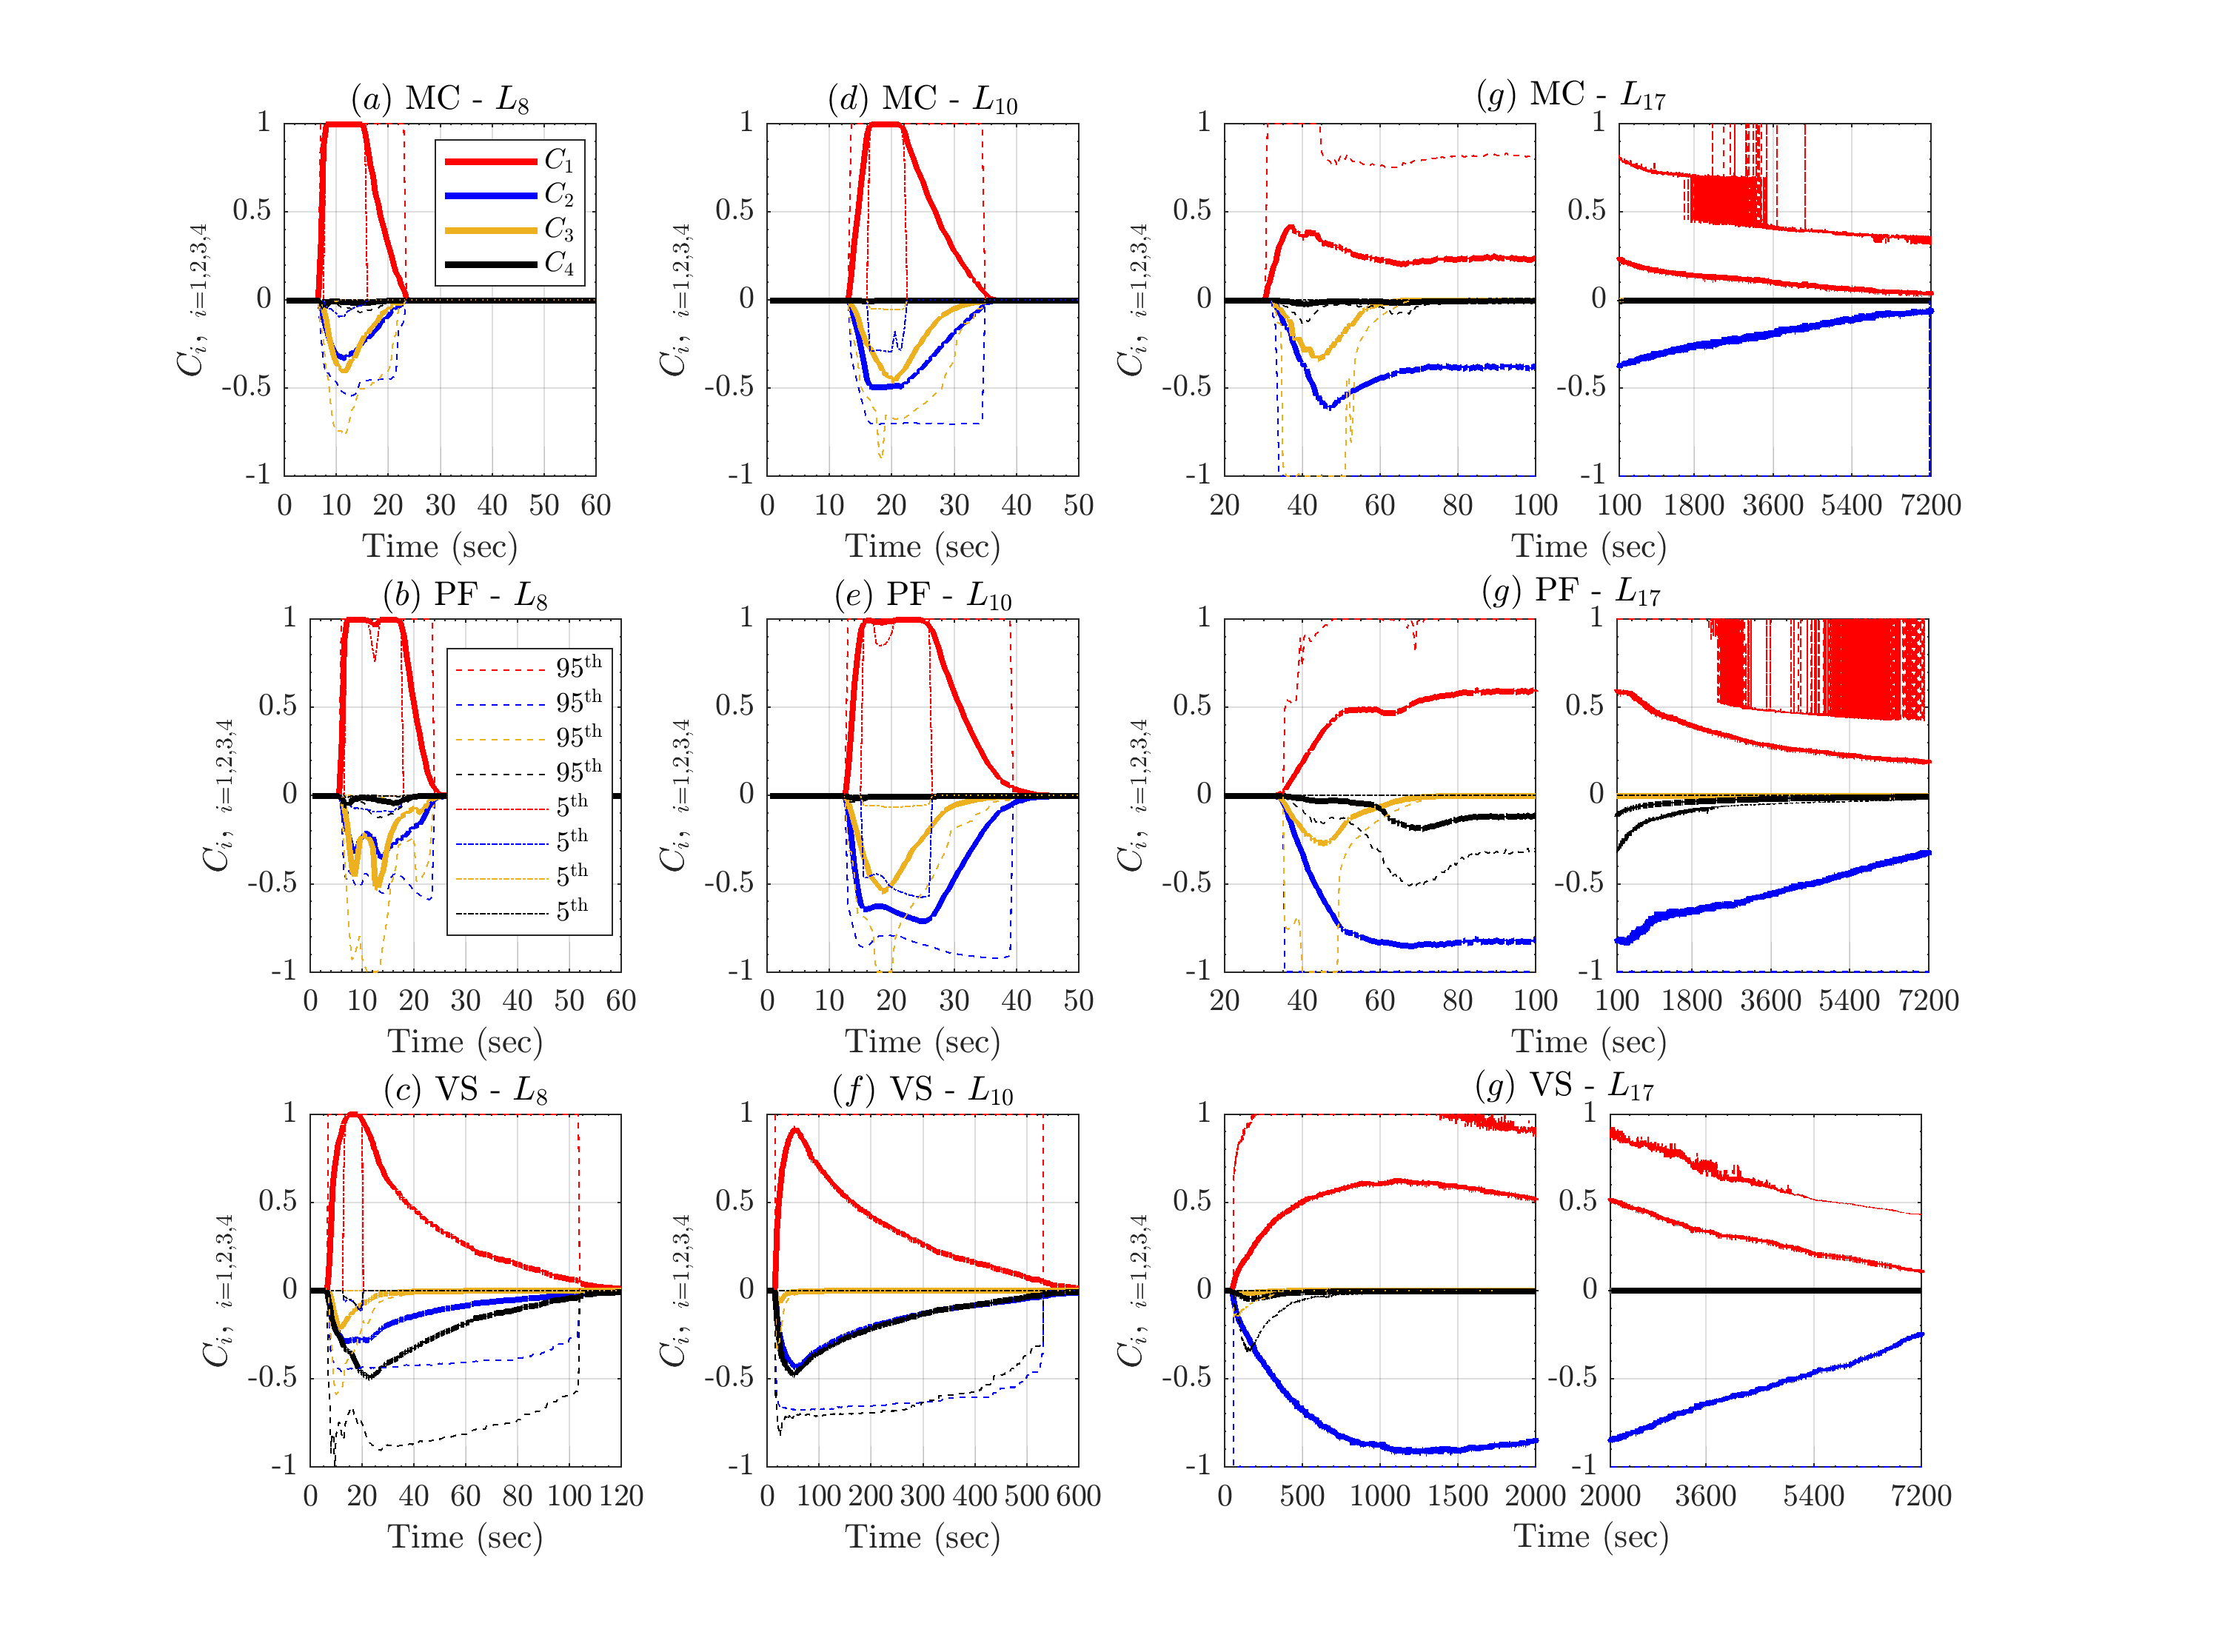
\includegraphics[width=1\textwidth]{BAF_VolcanDeColima/ForceContrib/Ci1_total.png}
        \caption{Records of contribution coefficients of \textbf{RHS} force moduli, at three spatial locations of interest, in the first km of runout. Different rheology models are displayed with different colors. Dominant factor is calculated based on the $l^\infty$ norm}
        \label{fig:Colima-Ci_1}
\end{figure}
The coefficients in the first two locations, points $L_8$ and $L_{10}$, are shown in \ref{fig:Colima-Ci_1}a,b,c and \ref{fig:Colima-Ci_1}d,e,f, respectively. Those points are close to the initial pile, in the western and eastern sectors of the inundated area. The pairs of plots related to the same model are similar. In all the models the greater contribution is given by $C_1$, significantly larger than $C_2$ and $C_3$, which have similar scales in MC and PF, while $C_2>C_3$ in VS.. $C_4$ always gives a negligible contribution, except for in VS, where it is comparable with $C_2$. In $L_8$, following PF, $C_3$ is bimodal, whereas the plot is unimodal in MC and VS, or in $L_{10}$. In $L_8$, $C_3$ is greater than in $L_{10}$, compared to the other forces. Like in the previous figures, VS shows a slower decrease of the plots, which is due to the rising probability of no-flow (see also next section). In plots \ref{fig:Colima-Ci_1}g,h,i, are shown the coefficients in $L_{17}$, about 1 km from the initial pile (in horizontal projection). The plots are split in two sub-frames, following different temporal scales - the first $100 s$ are on the left, and the rest of the temporal domain $[100, 7200] s$ is on the right. Initial dynamics is dominated by $C_2$, except for in MC, and only for a short time, $[30, 35] s$. In MC there is an initial peak of $C_2$ which is not observed in the other models.  $C_3$ has a significant size, in MC and PF, and unimodal profile. In PF, after $C_3$ wanes, at about $60 s$, also $C_4$, representing the effect of hydrostatic pressure correction, is not negligible, for $\sim 40 s$. The second part of the temporal domain, is characterized by a slow decrease of $C_2>C_1$, due to the rise of the no-flow probability.



















